\documentclass[14pt]{extreport}
\usepackage[utf8]{inputenc}
\usepackage[english, russian]{babel}
\usepackage{listings}
\usepackage{graphicx}
\usepackage{float}
\graphicspath{{imgs/}}
\usepackage{amsmath,amsfonts,amssymb,amsthm,mathtools} 
\usepackage{pgfplots}
\usepackage{filecontents}
\usepackage{indentfirst}
\usepackage{eucal}
\usepackage{enumitem}
\frenchspacing

\usepackage{indentfirst} % Красная строка

\usetikzlibrary{datavisualization}
\usetikzlibrary{datavisualization.formats.functions}

\usepackage{amsmath}
\usepackage{fixltx2e}
\usepackage{caption}


\definecolor{bluekeywords}{rgb}{0,0,1}
\definecolor{greencomments}{rgb}{0,0.5,0}
\definecolor{redstrings}{rgb}{0.64,0.08,0.08}
\definecolor{xmlcomments}{rgb}{0.5,0.5,0.5}
\definecolor{types}{rgb}{0.17,0.57,0.68}

\usepackage{listings}
\lstset{language=[Sharp]C,
	captionpos=t,
	numbers=left, %Nummerierung
	numberstyle=\small, % kleine Zeilennummern
	frame=single, % Oberhalb und unterhalb des Listings ist eine Linie
	stepnumber=1,                   
	numbersep=5pt,                
	showspaces=false,
	tabsize=2,
	showtabs=false,
	breaklines=true,
	showstringspaces=false,
	breakatwhitespace=true,
	escapeinside={(*@}{@*)},
	commentstyle=\color{greencomments},
	morekeywords={partial, var, value, get, set},
	keywordstyle=\color{bluekeywords},
	stringstyle=\color{redstrings},
	basicstyle=\ttfamily\small,
}

\usepackage[left=1cm,right=1cm, top=1cm,bottom=2cm,bindingoffset=0cm]{geometry}
% Для измененных титулов глав:
\usepackage{titlesec, blindtext, color} % подключаем нужные пакеты
\definecolor{gray75}{gray}{0.75} % определяем цвет
\newcommand{\hsp}{\hspace{20pt}} % длина линии в 20pt
% titleformat определяет стиль
\titleformat{\chapter}[hang]{\Huge\bfseries}{\thechapter\hsp\textcolor{gray75}{|}\hsp}{0pt}{\Huge\bfseries}

\usepackage{array}
\newcommand{\head}[2]{\multicolumn{1}{>{\centering\arraybackslash}p{#1}}{#2}}

% plot
\usepackage{pgfplots}
\usepackage{filecontents}
\usetikzlibrary{datavisualization}
\usetikzlibrary{datavisualization.formats.functions}

\begin{document}
	%\def\chaptername{} % убирает "Глава"
	\thispagestyle{empty}
	\begin{titlepage}
		\noindent \begin{minipage}{0.15\textwidth}
			
\includegraphics[width=\linewidth]{b_logo}
		\end{minipage}
		\noindent\begin{minipage}{0.9\textwidth}\centering
			\textbf{Министерство науки и высшего образования Российской Федерации}\\
			\textbf{Федеральное государственное бюджетное образовательное учреждение высшего образования}\\
			\textbf{~~~«Московский государственный технический университет имени Н.Э.~Баумана}\\
			\textbf{(национальный исследовательский университет)»}\\
			\textbf{(МГТУ им. Н.Э.~Баумана)}
		\end{minipage}
		
		\noindent\rule{18cm}{3pt}
		\newline\newline
		\noindent ФАКУЛЬТЕТ $\underline{~~~~~~~~~~~~~~~~~~~~~~~~~~~~~~~\text{«Информатика и системы управления»}~~~~~~~~~~~~~~~~~~~~~~~~~~~~~~~~~~~~~}$ \newline\newline
		\noindent КАФЕДРА $\underline{~~~~~~~~~~~~~\text{«Программное обеспечение ЭВМ и информационные технологии»}~~~~~~~~~~~~~~~~~~~~~~~}$\newline\newline\newline\newline\newline\newline
		
		
		\begin{center}
			\noindent\begin{minipage}{1.3\textwidth}\centering
				\Large\textbf{  Отчет по лабораторной работе №5}\newline
				\textbf{по дисциплине \newline "Моделирование"}\newline\newline
			\end{minipage}
		\end{center}
		
		\noindent\textbf{Тема} $\underline{\text{Моделирование работы информационного центра}}$\newline\newline
		\noindent\textbf{Студент} $\underline{\text{Малышев И. А.}}$\newline\newline
		\noindent\textbf{Группа} $\underline{\text{ИУ7-71Б}}$\newline\newline
		\noindent\textbf{Оценка (баллы)} $\underline{\text{~~~~~~~~~~~~~~~~~~~~~~~~~~~}}$\newline\newline
		\noindent\textbf{Преподаватель: } $\underline{\text{Рудаков И. В.}}$\newline\newline\newline
		
		\begin{center}
			\vfill
			Москва~---~\the\year
			~г.
		\end{center}
	\end{titlepage}
	
	
	\setcounter{page}{2}

\chapter{Задание}

В информационный центр приходят клиенты через интервал времени 10 ± 2 минуты. Если все три имеющихся оператора заняты, клиенту отказывают в обслуживании. Операторы имеют разную производительность и могут обеспечивать обслуживание среднего запроса пользователя за 20 ± 5; 40 ± 10; 40 ± 20. Клиенты стремятся занять свободного оператора с максимальной производительностью. Полученные запросы сдаются в накопитель. Откуда выбираются на обработку. На первый компьютер запросы от 1 и 2-ого операторов, на второй -- запросы от 3-его. Время обработки запросов первым и 2- м компьютером равны соответственно 15 и 30 мин. Промоделировать процесс обработки 300 запросов.

Для выполнения поставленного задания необходимо создать концептуальную модель в терминах СМО, определить эндогенные и экзогенные переменные и уравнения модели. За единицу системного времени выбрать 0.01 минуты.

\chapter{Решение}
\section{Теоретическая часть}

\subsection{Концептуальная модель системы в терминах СМО}

На рисунке \ref{img:model} предоставлена концептуальная модель моделируемой системы в терминах СМО.

\begin{figure}[H]
	\begin{center}
		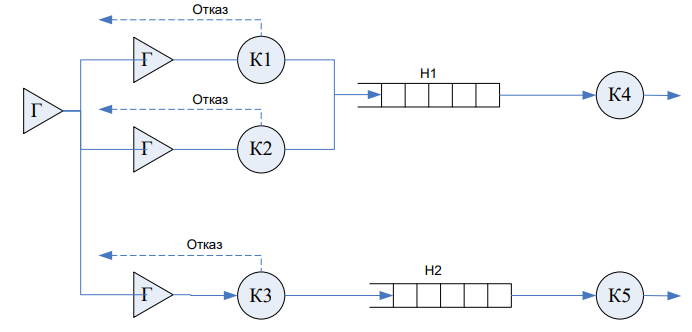
\includegraphics[scale=0.9]{imgs/model.png}
	\end{center}
	\caption{Концептуальная модель системы в терминах СМО.}
	\label{img:model}
\end{figure}

В процессе взаимодействия клиентов с информационным центром возможен.

\begin{enumerate}
	\item Режим нормального обслуживания, т.е. клиент выбирает одного из свободных операторов, отдавая предпочтение тому у которого меньше номер.
	\item Режим отказа в обслуживании клиента, когда все операторы заняты.
\end{enumerate}

\subsection{Переменные и уравнения имитационной модели}

Эндогенные переменные: время обработки задания i-ым оператором, время решения этого задания j-ым компьютером.

Экзогенные переменные: число обслуженных клиентов и число клиентов, получивших отказ.

Вероятность отказа в обслуживании клиента:

\begin{equation}
	P_{отк} = \frac{C_{refus}}{C_{refus} + C_{serv}},
\end{equation}

где $C_{refus}$ -- количество заявок, которым было отказано в обслуживании, $C_{serv}$ -- – количество заявок, которые были обслужены.

\section{Листинг}

Далее представлен фрагмент программы, выполняющий поставленное задание.

\begin{lstlisting}
using Generator = Func<double>;

internal interface Processor
{
	bool GetRequest();
}

static class ModelTimer
{
	public static double CurrentTime { get; set; } = 0;
}

class RequestGenerator
{
	Generator generator;
	public int numberOfGeneratedRequests;
	public double timeOfNextEvent;
	List<Processor> receivers;
	
	public RequestGenerator(Generator generator)
	{
		this.generator = generator;
		numberOfGeneratedRequests = 0;
		receivers = new List<Processor>();
		timeOfNextEvent = 0;
	}
	
	public void SubscribeReceiver(Processor receiver) 
	{
		receivers.Add(receiver);
	}
	
	public double GetNextTime() => generator();
	
	public Processor SendRequest()
	{
		numberOfGeneratedRequests++;
		foreach (var receiver in receivers)
		{
			if (receiver.GetRequest())
			return receiver;
		}
		
		return null;
	}
}

class RequestProcessor: RequestGenerator, Processor
{
	public int numberOfRequestsInQueue, numberOfProcessedRequests;
	int maxOfQueue;
	
	public RequestProcessor(Generator generator, int maxOfQueue = 0) : base(generator)
	{
		numberOfRequestsInQueue = 0;
		numberOfProcessedRequests = 0;
		this.maxOfQueue = maxOfQueue;
	}
	
	public void Process()
	{
		if (numberOfRequestsInQueue > 0)
		{
			numberOfProcessedRequests++;
			numberOfRequestsInQueue--;
			SendRequest();
		}
		
		timeOfNextEvent = numberOfRequestsInQueue > 0 ? ModelTimer.CurrentTime + GetNextTime() : 0.0;
	}
	
	public bool GetRequest()
	{
		if (maxOfQueue == 0 || numberOfRequestsInQueue < maxOfQueue)
		{
			numberOfRequestsInQueue++;
			if (timeOfNextEvent == 0)
			timeOfNextEvent = ModelTimer.CurrentTime + GetNextTime();
			
			return true;
		}
		else
		return false;
	}
}

struct SimulationParameters
{
	public Client client;
	public Operator operator1, operator2, operator3;
	public Computer computer1, computer2;
	
	public SimulationParameters(Client client, Operator operator1, Operator operator2, Operator operator3, Computer computer1, Computer computer2)
	{
		this.client = client;
		this.operator1 = operator1;
		this.operator2 = operator2;
		this.operator3 = operator3;
		this.computer1 = computer1;
		this.computer2 = computer2;
	}
}

struct Client
{
	public int timeOfCome, timeDelta, amountOfProccessedNeeded;
	
	public Client(int timeOfCome, int timeDelta, int amountOfProccessedNeeded)
	{
		this.timeDelta = timeDelta;
		this.timeOfCome = timeOfCome;
		this.amountOfProccessedNeeded = amountOfProccessedNeeded;
	}
}

struct Operator
{
	public int timeOfService, timeDelta;
	
	public Operator(int timeOfService, int timeDelta)
	{
		this.timeOfService = timeOfService;
		this.timeDelta = timeDelta;
	}
}

struct Computer
{
	public int timeOfService;
	
	public Computer(int timeOfService) 
	{
		this.timeOfService = timeOfService;
	}
}

struct Results
{
	public int numberOfDenials;
	public double probabilityOfDenial;
	
	public Results(int numberOfDenials, double probabilityOfDenial)
	{
		this.numberOfDenials = numberOfDenials;
		this.probabilityOfDenial = probabilityOfDenial;
	}
	
	public static Results DoSimulate(SimulationParameters parameters)
	{
		RequestGenerator generatorOfClients = new RequestGenerator(() => 
		UniformDistributions.GetUniformReal(
		parameters.client.timeOfCome - parameters.client.timeDelta,
		parameters.client.timeOfCome + parameters.client.timeDelta));
		
		RequestProcessor operator1 = new RequestProcessor(() => 
		UniformDistributions.GetUniformReal(
		parameters.operator1.timeOfService - parameters.operator1.timeDelta,
		parameters.operator1.timeOfService + parameters.operator1.timeDelta), 1);
		
		RequestProcessor operator2 = new RequestProcessor(() =>  
		UniformDistributions.GetUniformReal(
		parameters.operator2.timeOfService - parameters.operator2.timeDelta,
		parameters.operator2.timeOfService + parameters.operator2.timeDelta), 1);
		
		RequestProcessor operator3 = new RequestProcessor(() => 
		UniformDistributions.GetUniformReal(
		parameters.operator3.timeOfService - parameters.operator3.timeDelta,
		parameters.operator3.timeOfService + parameters.operator3.timeDelta), 1);
		
		RequestProcessor computer1 = new RequestProcessor(() => parameters.computer1.timeOfService);
		RequestProcessor computer2 = new RequestProcessor(() => parameters.computer2.timeOfService);
		
		generatorOfClients.SubscribeReceiver(operator1);
		generatorOfClients.SubscribeReceiver(operator2);
		generatorOfClients.SubscribeReceiver(operator3);
		
		operator1.SubscribeReceiver(computer1);
		operator2.SubscribeReceiver(computer1);
		operator3.SubscribeReceiver(computer2);
		
		RequestGenerator[] schemeElements = new RequestGenerator[]{
			generatorOfClients, operator1, operator2, operator3, computer1, computer2};
		
		int numberOfDenials = 0;
		generatorOfClients.timeOfNextEvent = generatorOfClients.GetNextTime();
		
		while (computer1.numberOfProcessedRequests + computer2.numberOfProcessedRequests <
		parameters.client.amountOfProccessedNeeded)
		{
			ModelTimer.CurrentTime = generatorOfClients.timeOfNextEvent;
			foreach (var element in schemeElements)
			{
				if (element.timeOfNextEvent != 0 && element.timeOfNextEvent < ModelTimer.CurrentTime)
				{
					ModelTimer.CurrentTime = element.timeOfNextEvent;
				}
			}
			
			foreach (var element in schemeElements)
			{
				if (ModelTimer.CurrentTime == element.timeOfNextEvent)
				{
					RequestProcessor processor = element as RequestProcessor;
					if (processor is not null)
						processor.Process();
					else
					{
						Processor catchProcessor = generatorOfClients.SendRequest();
						if (catchProcessor is null)
						numberOfDenials++;
						
						generatorOfClients.timeOfNextEvent = ModelTimer.CurrentTime + generatorOfClients.GetNextTime();
					}
				}
			}
		}
		
		return new Results(numberOfDenials, numberOfDenials / ((double)numberOfDenials + operator1.numberOfProcessedRequests +
		operator2.numberOfProcessedRequests +
		operator3.numberOfProcessedRequests));
	}
}

static class UniformDistributions
{
	public static double GetUniformReal(double aParameter, double bParameter)
	{
		return ContinuousUniform.Sample(aParameter, bParameter);
	}
	
	public static int GetUniformInt(int aParameter, int bParameter) 
	{
		return (int)Math.Round(ContinuousUniform.Sample(aParameter, bParameter));
	}
}
\end{lstlisting}

\section{Результаты работы}

Моделирование проводилось с использованием событийного принципа.

Важно отметить, что в силу того, что система подразбита на два <<домена>>, вычисляемая вероятность отказа прямо не зависит от скорости обработки запросов компьютеров, которая позволяют лишь увеличить или уменьшить время моделирования системы, так как конечным условием моделирования является обработка 300 запросов. В качестве количества обслуженных заявок бралась сумма обработанных операторами заявок.

На рисунке \ref{img:ui} представлен пользовательский интерфейс программы в исходном состоянии.

\begin{figure}[H]
	\begin{center}
		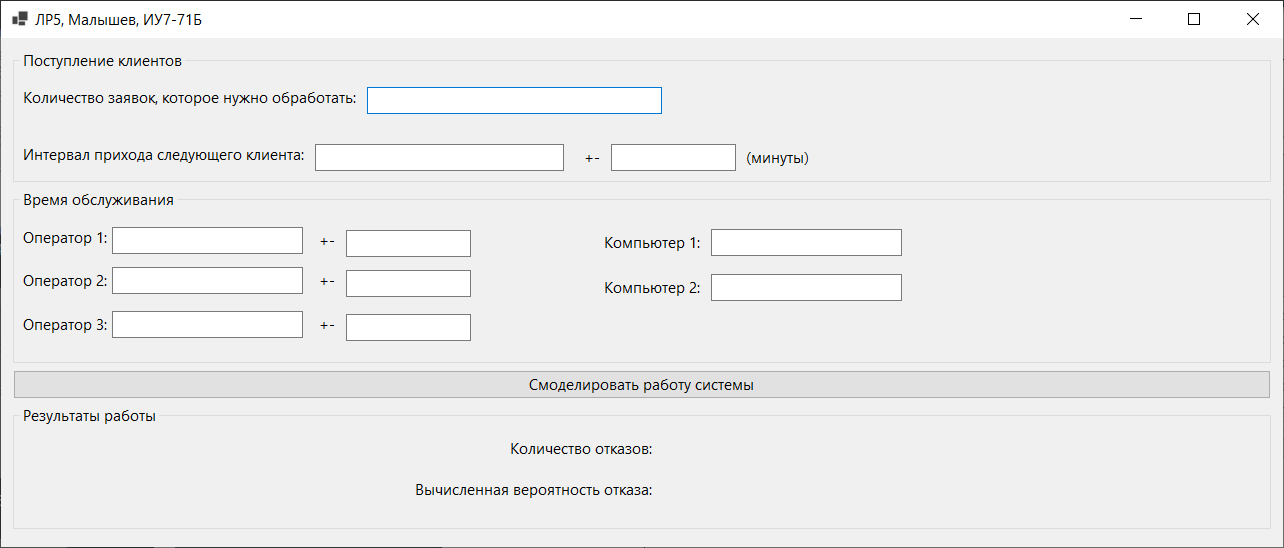
\includegraphics[scale=0.8]{imgs/ui.png}
	\end{center}
	\caption{Пользовательский интерфейс программы в исходном состоянии.}
	\label{img:ui}
\end{figure}

На рисунках \ref{img:res1}-\ref{img:res2} представлены примеры результатов работы программы с указанными данными.

\begin{figure}[H]
	\begin{center}
		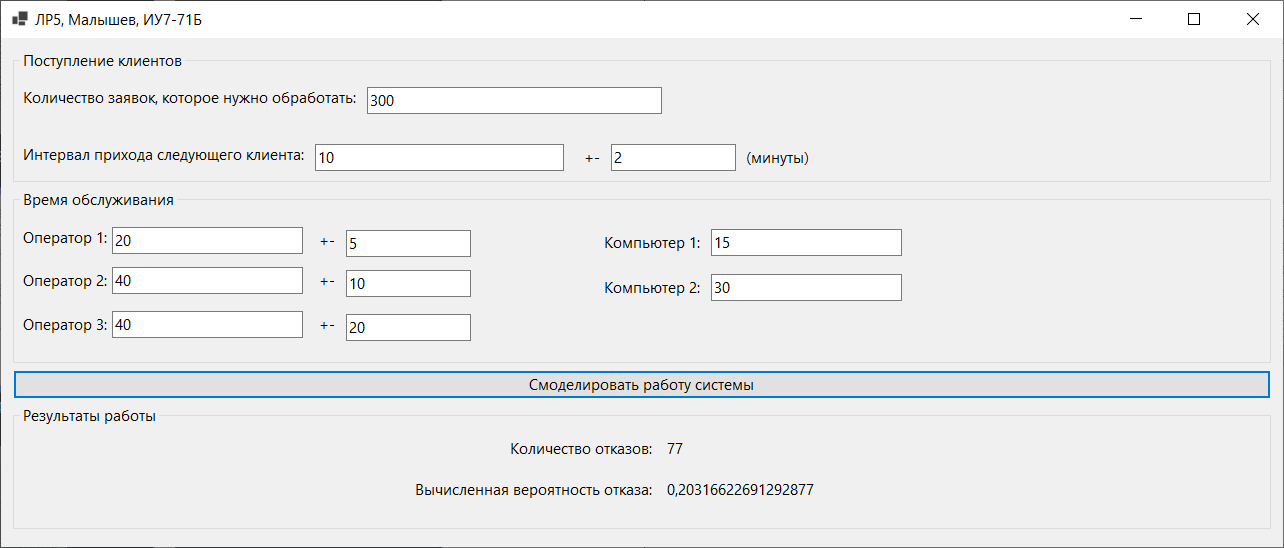
\includegraphics[scale=0.8]{imgs/res1.png}
	\end{center}
	\caption{Пример работы реализованного приложения.}
	\label{img:res1}
\end{figure}

\begin{figure}[H]
	\begin{center}
		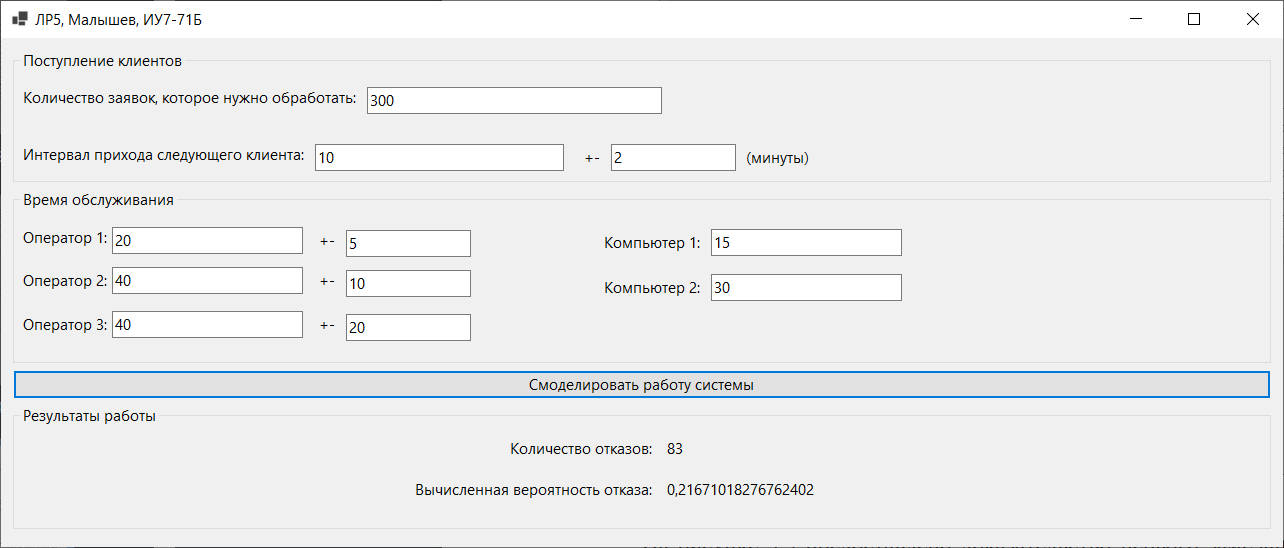
\includegraphics[scale=0.8]{imgs/res2.png}
	\end{center}
	\caption{Пример работы реализованного приложения.}
	\label{img:res2}
\end{figure}

На рисунке \ref{img:res3} предоставлено доказательство первого замечания. Как видно, вычисленная вероятность отказа остаётся примерно такой же, как и на предыдущих данных.

\begin{figure}[H]
	\begin{center}
		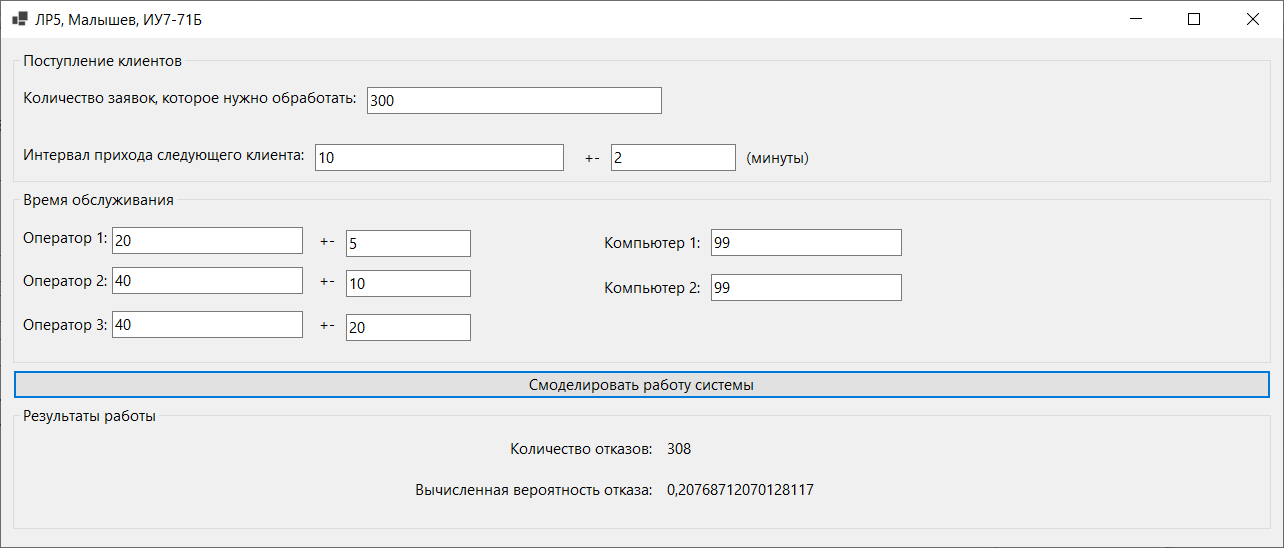
\includegraphics[scale=0.8]{imgs/res3.png}
	\end{center}
	\caption{Значительное уменьшение скорости обработки запросов компьютерами.}
	\label{img:res3}
\end{figure}

\end{document}